

\section{Results}
Our approach performs well on real data even facing occlusions and clutter in the indoor enviroment. A visual sample is shown in Fig. \ref{fig:results1}. The first row are the input multi-view images, the second row are the predicted probability maps from the network. We do the same prediction on the flipped version of the input images and average the corresponding probability maps. Then the predictions from different views are merged to generate the overall probability map on the left of the third row, and the final result is on its right. In this scene, 12 images from different horizontal perspectives are used. Note that several secondary keypoints are occluded by objects, such as the keypoints behind the bed and the TV, but we can still recover the overall layout of the room properly. Our method also show robustness to clutter, such as the many small objects around the TV. (maybe more visual results and analysis)

\begin{figure}[ht]
	\centering
	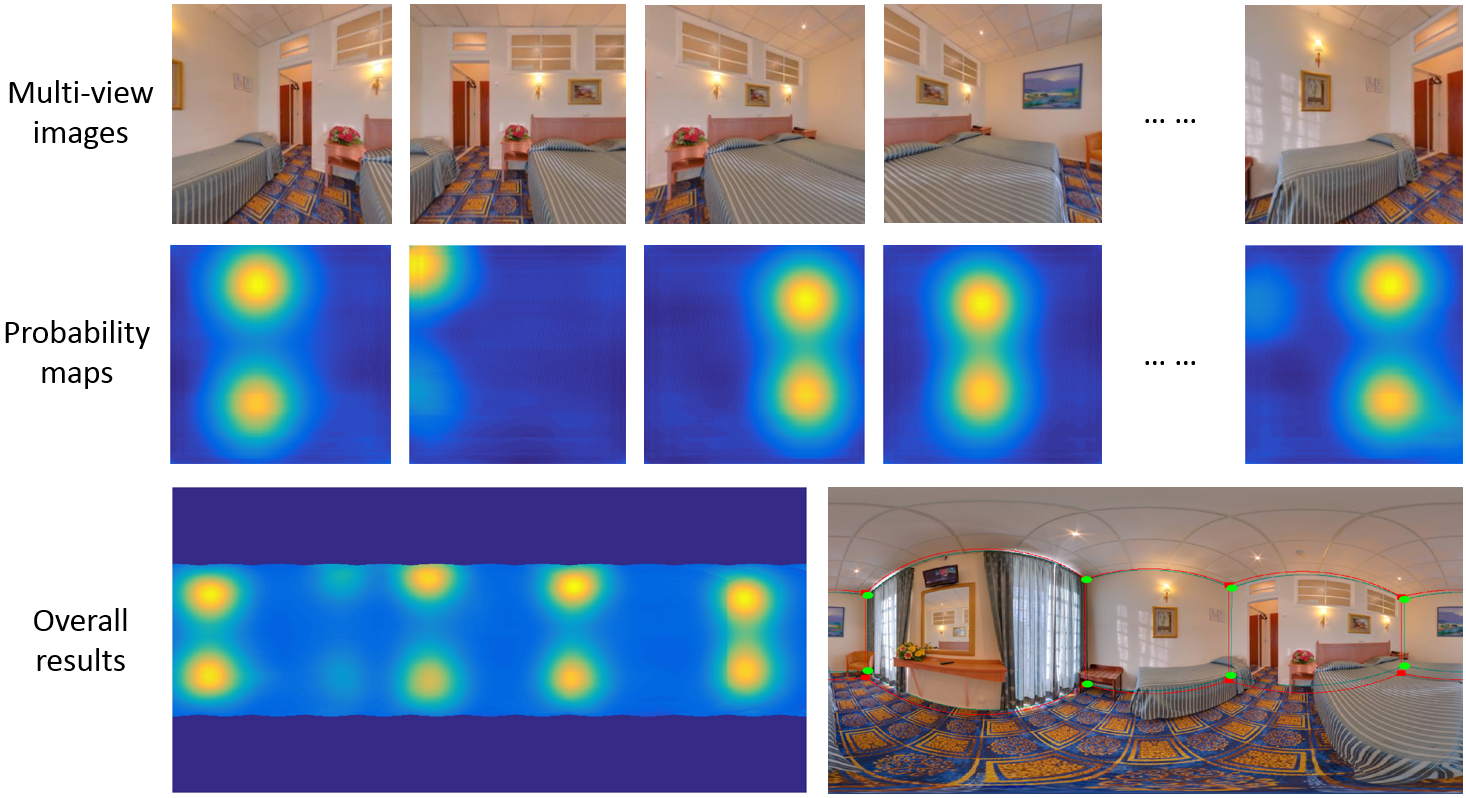
\includegraphics[width=\linewidth]{figs/results2.png}
	\caption{Our qualitative results on real data. We sum over the third dimension of the probability array $T$ for visulization. In the final result, the ground truth is shown in green and our prediction is shown in red. }
	\label{fig:results2}
\end{figure}

\begin{figure}
	\centering
	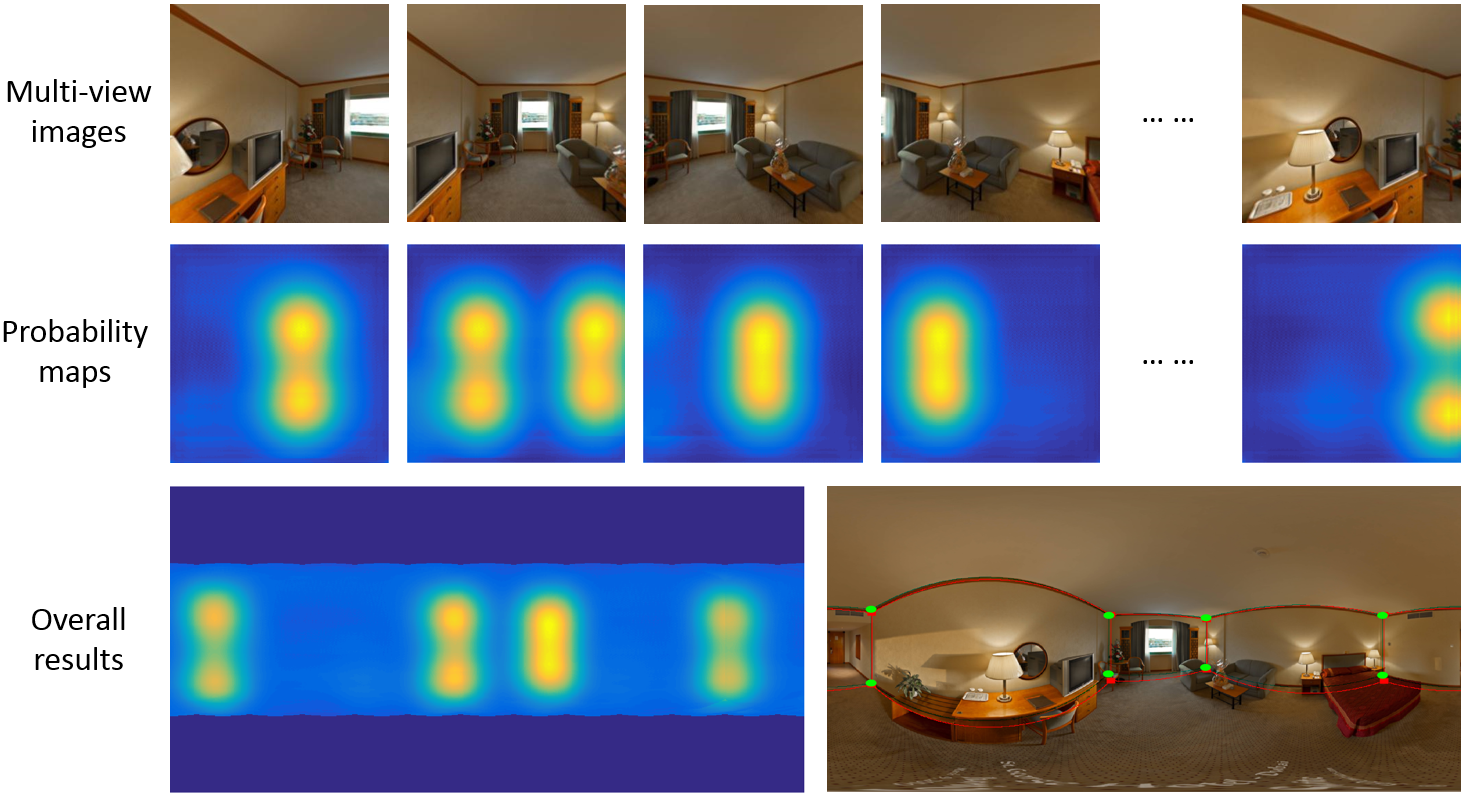
\includegraphics[width=\linewidth]{figs/results3.png}
	\caption{alternative/more results. }
	\label{fig:results3}
\end{figure}

\begin{figure}
	\centering
	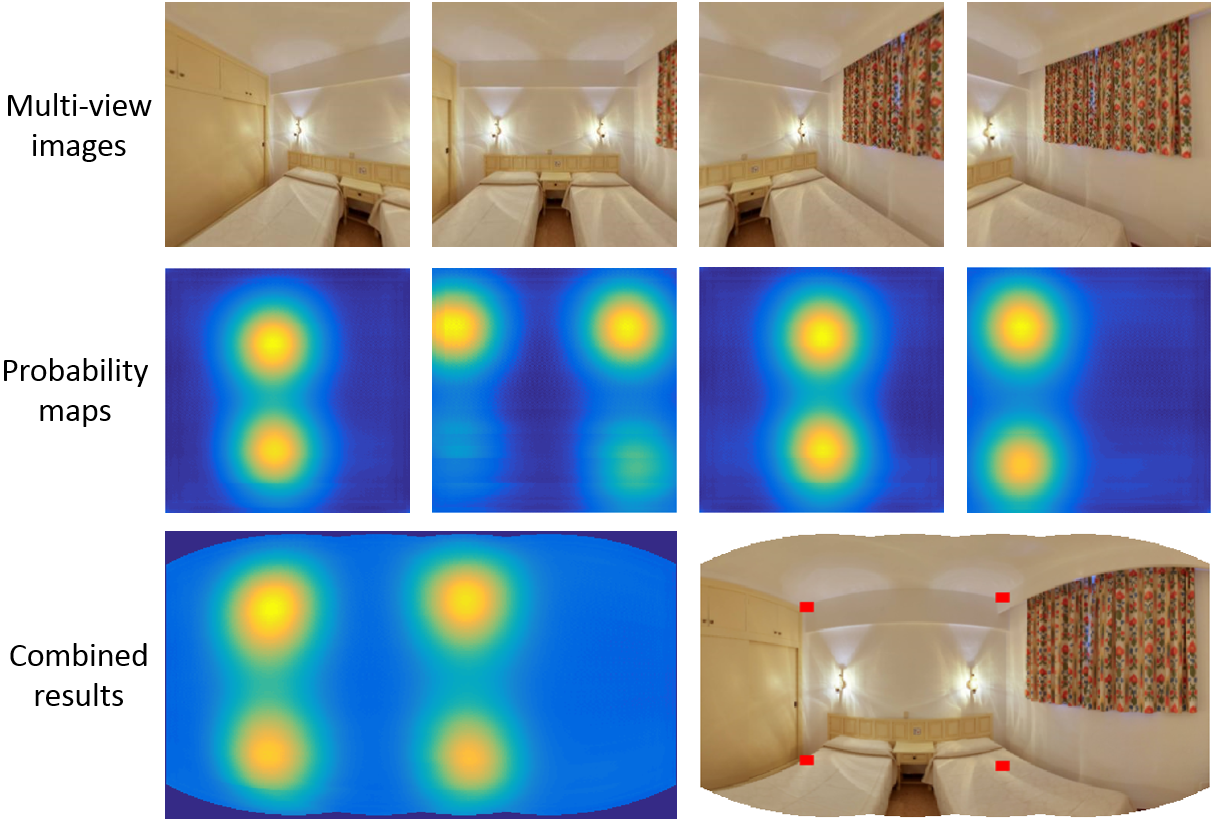
\includegraphics[width=\linewidth]{figs/partial1.png}
	\caption{the results of the combined partial views. }
	\label{fig:partial1}
\end{figure}

\begin{figure}
	\centering
	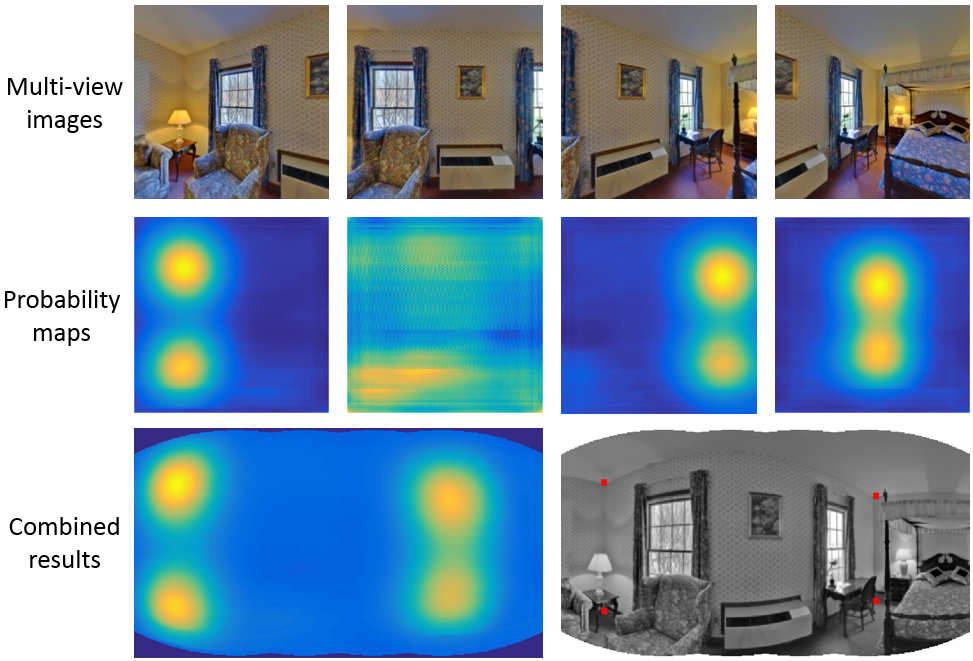
\includegraphics[width=\linewidth]{figs/partial2.png}
	\caption{alternative/more results of the combined partial views. }
	\label{fig:partial2}
\end{figure}


We also conduct experiments on the PanoContext dataset for quantitive comparison with previous panorama based methods, the same training/testing split is adopted. Three standard metrics are adopted for evaluation: 3D Intersection over Union, Corner error and Pixel error. As shown in Tab. \ref{tab:PC}, our approach is nearly on par with the panorama based methods. We believe that the reason for this deficiency is that the FOV of each perspective image is much smaller than that of the panorama. Limited FOV may lead to the wrong focus, as shown in Fig. \ref{wrong}, which then pollutes the overall prediction. To explore the effect of using different size of FOV, we use two different settings during training and testing. For \ang{60}, we project the panorama into 24 perspective images with $FOV=\ang{60}$, while 8 directions around the vertical axis and 3 directions around the horizontal axis. For \ang{90}, we project the panorama into 12 perspective images with $FOV=\ang{90}$, all of them are horizontal and centered around the vertical axis. The quantitative results in Tab. \ref{tab:PC} demonstrate that larger FOV contribute to higher accuracy in overall prediction, which is also consistent with our intuition. In fact, the panorama can be viewed as a special case that the FOV reaches its maximum.


%Experiments, three parts: one for different field of view (FOV), one for comparison with panorama based method, the last one for qualitative results.


%\begin{table}
%	\caption{Results of different FOV.}
%	\label{tab:FOV}
%	\begin{tabular}{cccc}
%		\toprule
%		FOV &3D IoU (\%)&Corner error (\%)&Pixel error (\%)\\
%		\midrule
%		 \ang{60} & XX & XX & XX\\
%	     \ang{90} & XX & XX & XX\\	
%		\bottomrule
%	\end{tabular}
%\end{table}


\begin{table}
	\caption{Quantitative results on PanoContext dataset.}
	\label{tab:PC}
	\begin{tabular}{cccc}
		\toprule
		Method&3D IoU (\%)& $\epsilon_{corner}$ (\%) & $\epsilon_{pixel}$ (\%)\\
		\midrule
		PanoContext \cite{zhang2014panocontext} & 67.23 & 1.60 & 4.55\\
		LayoutNet \cite{zou2018layoutnet} & 74.48 & 1.06 & 3.34\\
		Our Method \ang{60} & XX & XX & XX\\	
		Our Method \ang{90} & 59.58 & 2.20 & 6.78\\	
		\ang{90} add flip & 61.98 & 2.75 & 6.73\\	
		\bottomrule
	\end{tabular}
\end{table}

\section{Conclusions}
In this paper, we propose a method to estimate the overall room layout based on multiple views. We design a secondary representation for the room layout in the perspective image to simplify the learning process. Then we integrate the predicted room layout from different perpectives into a holistic prediction using image stitching and a fusion strategy. Our output panoramic results can be further rendered into a 3D representation. This is an encouraging attempt to estimate the whole room layout using multiple perspectives and without using structure from motion.

\comments{
\begin{acks}
	The authors would like to thank ...
\end{acks}
}